\documentclass[11pt,a4paper]{article}

\usepackage[utf8]{inputenc}
\usepackage[T1]{fontenc}
\usepackage{babel}
\babelprovide[import,main]{indonesian}
\usepackage{amsmath,amssymb,amsthm}
\usepackage[margin=2.5cm]{geometry}
\usepackage{tikz}
\usepackage{xcolor}
\usepackage{tcolorbox}
\usepackage{enumitem}
\usepackage{hyperref}

\tcbuselibrary{skins,breakable}

\newtcolorbox{soal}{colback=blue!5,colframe=blue!50!black,title=Soal,fonttitle=\bfseries,breakable}
\newtcolorbox{jawaban}{colback=green!5,colframe=green!45!black,fonttitle=\bfseries,title=Jawaban Akhir}
\newtcolorbox{catatan}{colback=orange!5,colframe=orange!70!black,fonttitle=\bfseries,title=Catatan,breakable}

\setlength{\parindent}{0pt}
\setlength{\parskip}{6pt}

\title{\textbf{Pembahasan Soal Fungsi Densitas Bersama}\\[4pt]
\large Densitas Marginal, Densitas Bersyarat, dan Nilai Harapan Bersyarat}
\author{}
\date{}

\begin{document}
\maketitle

\begin{soal}
Misalkan variabel random $X$ dan $Y$ mempunyai fungsi densitas bersama
\[
f(x,y)=
\begin{cases}
Cxy, & 0<y<x<1\\[2pt]
0, & \text{lainnya}
\end{cases}
\]
\begin{enumerate}[leftmargin=*]
  \item Tentukan nilai $C$ sedemikian sehingga $f(x,y)$ merupakan fungsi densitas bersama.
  \item Tentukan densitas marginal $f(x)$.
  \item Tentukan fungsi densitas bersyarat $f(y\mid x)$.
  \item Tentukan nilai harapan bersyarat $E\!\left(Y\mid X=\tfrac13\right)$.
\end{enumerate}
\end{soal}

%==================================================
\section*{Persiapan: Memahami Daerah Definisi}

Fungsi densitas bernilai tak nol hanya pada daerah
\[
D=\{(x,y): 0<y<x<1\}.
\]
Daerah ini adalah segitiga dengan titik sudut $(0,0)$, $(1,0)$, dan $(1,1)$, yaitu bagian persegi satuan yang berada \emph{di bawah} garis $y=x$.

\begin{center}
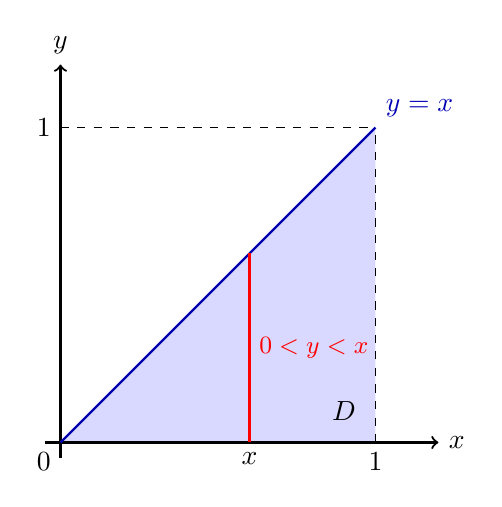
\begin{tikzpicture}[scale=4]
  \fill[blue!15] (0,0) -- (1,0) -- (1,1) -- cycle;
  \draw[->,thick] (-0.05,0) -- (1.2,0) node[right] {$x$};
  \draw[->,thick] (0,-0.05) -- (0,1.2) node[above] {$y$};
  \draw[thick,blue!70!black] (0,0) -- (1,1) node[above right] {$y=x$};
  \draw[dashed] (1,0) -- (1,1);
  \draw[dashed] (0,1) -- (1,1);
  \node[below] at (1,0) {$1$};
  \node[left] at (0,1) {$1$};
  \node[below left] at (0,0) {$0$};
  % irisan vertikal
  \draw[very thick,red] (0.6,0) -- (0.6,0.6);
  \node[below] at (0.6,0) {$x$};
  \node[red,right] at (0.6,0.3) {\small $0<y<x$};
  \node at (0.9,0.1) {$D$};
\end{tikzpicture}
\end{center}

Untuk setiap $x$ tetap dengan $0<x<1$, nilai $y$ bergerak dari $0$ sampai $x$ (garis merah). Karena itu, saat mengintegralkan terhadap $y$ terlebih dahulu, batasnya adalah
\[
\int_{x=0}^{1}\int_{y=0}^{x} (\cdots)\,dy\,dx.
\]

\begin{catatan}
Kesalahan yang paling sering terjadi adalah memakai batas $0<x<1$ dan $0<y<1$ (seluruh persegi). Batas tersebut \textbf{salah}, karena syarat $y<x$ membuat daerahnya hanya setengah persegi.
\end{catatan}

%==================================================
\section*{1. Menentukan Nilai $C$}

\textbf{Konsep.} Suatu fungsi $f(x,y)$ adalah fungsi densitas bersama jika memenuhi dua syarat:
\begin{enumerate}[label=(\roman*)]
  \item $f(x,y)\ge 0$ untuk semua $(x,y)$,
  \item $\displaystyle\iint_{\mathbb{R}^2} f(x,y)\,dx\,dy = 1$.
\end{enumerate}

\textbf{Syarat (ii).}
\begin{align*}
\iint_D Cxy\,dA
&= \int_0^1\int_0^x Cxy\,dy\,dx \\[4pt]
&= C\int_0^1 x\left[\frac{y^2}{2}\right]_{y=0}^{y=x} dx \\[4pt]
&= C\int_0^1 x\cdot\frac{x^2}{2}\,dx
 = \frac{C}{2}\int_0^1 x^3\,dx \\[4pt]
&= \frac{C}{2}\left[\frac{x^4}{4}\right]_0^1
 = \frac{C}{2}\cdot\frac14
 = \frac{C}{8}.
\end{align*}
Agar total peluang sama dengan $1$:
\[
\frac{C}{8}=1 \quad\Longrightarrow\quad C=8.
\]

\textbf{Syarat (i).} Pada $D$ berlaku $x>0$ dan $y>0$, sehingga $8xy>0$. Di luar $D$, $f(x,y)=0$. Jadi $f(x,y)\ge 0$ terpenuhi.

\textbf{Verifikasi dengan urutan integrasi lain.} Jika $y$ ditetapkan terlebih dahulu, maka $0<y<1$ dan $y<x<1$:
\[
\int_0^1\int_y^1 8xy\,dx\,dy
= \int_0^1 8y\left[\frac{x^2}{2}\right]_y^1 dy
= \int_0^1 4y(1-y^2)\,dy
= 4\left(\frac12-\frac14\right)=1.\ \checkmark
\]

\begin{jawaban}
\[
C = 8, \qquad
f(x,y)=\begin{cases} 8xy, & 0<y<x<1\\ 0, & \text{lainnya}\end{cases}
\]
\end{jawaban}

%==================================================
\section*{2. Densitas Marginal $f(x)$}

\textbf{Konsep.} Densitas marginal $X$ diperoleh dengan mengintegralkan densitas bersama terhadap seluruh nilai $y$ yang mungkin:
\[
f_X(x)=\int_{-\infty}^{\infty} f(x,y)\,dy.
\]

\textbf{Perhitungan.} Untuk $0<x<1$, nilai $f(x,y)$ tak nol hanya ketika $0<y<x$:
\begin{align*}
f_X(x)
&= \int_0^x 8xy\,dy
 = 8x\left[\frac{y^2}{2}\right]_0^x
 = 8x\cdot\frac{x^2}{2}
 = 4x^3.
\end{align*}
Untuk $x\le 0$ atau $x\ge 1$, $f(x,y)=0$ untuk semua $y$, sehingga $f_X(x)=0$.

\textbf{Verifikasi.}
\[
\int_0^1 4x^3\,dx = \left[x^4\right]_0^1 = 1.\ \checkmark
\]

\begin{jawaban}
\[
f(x)=\begin{cases} 4x^3, & 0<x<1\\ 0, & \text{lainnya}\end{cases}
\]
\end{jawaban}

\begin{catatan}
Sebagai pelengkap, densitas marginal $Y$ adalah
\[
f_Y(y)=\int_y^1 8xy\,dx = 4y(1-y^2),\qquad 0<y<1.
\]
Perhatikan bahwa $f(x,y)=8xy \neq f_X(x)\,f_Y(y)=16x^3y(1-y^2)$, sehingga $X$ dan $Y$ \textbf{tidak saling bebas}. Hal ini juga terlihat dari daerah $D$ yang bukan berbentuk persegi panjang: nilai $X$ membatasi kemungkinan nilai $Y$.
\end{catatan}

%==================================================
\section*{3. Fungsi Densitas Bersyarat $f(y\mid x)$}

\textbf{Konsep.} Untuk $x$ dengan $f_X(x)>0$, densitas bersyarat $Y$ diberikan $X=x$ adalah
\[
f(y\mid x)=\frac{f(x,y)}{f_X(x)}.
\]

\textbf{Perhitungan.} Untuk $0<x<1$ dan $0<y<x$:
\[
f(y\mid x)=\frac{8xy}{4x^3}=\frac{2y}{x^2}.
\]

\textbf{Verifikasi} bahwa ini merupakan densitas (terhadap $y$) untuk setiap $x$ tetap:
\[
\int_0^x \frac{2y}{x^2}\,dy
= \frac{1}{x^2}\left[y^2\right]_0^x
= \frac{x^2}{x^2}=1.\ \checkmark
\]

\begin{jawaban}
Untuk setiap $0<x<1$,
\[
f(y\mid x)=\begin{cases} \dfrac{2y}{x^2}, & 0<y<x\\[6pt] 0, & \text{lainnya}\end{cases}
\]
\end{jawaban}

\begin{catatan}
Interpretasi: diberikan $X=x$, variabel $Y$ hanya dapat bernilai di $(0,x)$ dan densitasnya naik secara linear terhadap $y$. Artinya, nilai $Y$ yang mendekati $x$ lebih mungkin muncul dibandingkan nilai $Y$ yang mendekati $0$.
\end{catatan}

%==================================================
\section*{4. Nilai Harapan Bersyarat $E\!\left(Y\mid X=\tfrac13\right)$}

\textbf{Konsep.}
\[
E(Y\mid X=x)=\int_{-\infty}^{\infty} y\,f(y\mid x)\,dy.
\]

\subsection*{Cara 1: Rumus umum, lalu substitusi}
\begin{align*}
E(Y\mid X=x)
&= \int_0^x y\cdot\frac{2y}{x^2}\,dy
 = \frac{2}{x^2}\int_0^x y^2\,dy \\[4pt]
&= \frac{2}{x^2}\left[\frac{y^3}{3}\right]_0^x
 = \frac{2}{x^2}\cdot\frac{x^3}{3}
 = \frac{2x}{3}.
\end{align*}
Substitusi $x=\tfrac13$:
\[
E\!\left(Y\mid X=\tfrac13\right)=\frac23\cdot\frac13=\frac29.
\]

\subsection*{Cara 2: Langsung dari densitas bersyarat di $x=\tfrac13$}
Dengan $x=\tfrac13$, diperoleh $x^2=\tfrac19$, sehingga
\[
f\!\left(y\mid \tfrac13\right)=\frac{2y}{1/9}=18y,\qquad 0<y<\tfrac13.
\]
(Cek: $\int_0^{1/3}18y\,dy = 9\cdot\tfrac19 = 1$ \checkmark.) Maka
\begin{align*}
E\!\left(Y\mid X=\tfrac13\right)
&= \int_0^{1/3} y\cdot 18y\,dy
 = 18\left[\frac{y^3}{3}\right]_0^{1/3}
 = 6\cdot\frac{1}{27}
 = \frac{2}{9}.
\end{align*}

\begin{jawaban}
\[
E(Y\mid X=x)=\frac{2x}{3},\qquad
E\!\left(Y\mid X=\tfrac13\right)=\frac{2}{9}\approx 0{,}2222.
\]
\end{jawaban}

\begin{catatan}
\textbf{Cek kewajaran.} Diberikan $X=\tfrac13$, nilai $Y$ berada di $(0,\tfrac13)$, sehingga ekspektasinya pasti berada di interval tersebut. Hasil $\tfrac29\approx0{,}222$ memang di dalam $(0,\,0{,}333)$, dan lebih besar dari titik tengah $\tfrac16\approx0{,}167$. Ini konsisten dengan interpretasi pada nomor 3: densitas bersyarat lebih berat ke arah nilai $y$ yang besar.
\end{catatan}

%==================================================
\section*{Ringkasan}

\begin{center}
\renewcommand{\arraystretch}{1.8}
\begin{tabular}{|c|l|c|}
\hline
\textbf{No.} & \textbf{Yang dicari} & \textbf{Hasil} \\
\hline
1 & Konstanta $C$ & $C=8$ \\
\hline
2 & Densitas marginal $f(x)$ & $4x^3,\ \ 0<x<1$ \\
\hline
3 & Densitas bersyarat $f(y\mid x)$ & $\dfrac{2y}{x^2},\ \ 0<y<x$ \\
\hline
4 & $E\!\left(Y\mid X=\tfrac13\right)$ & $\dfrac{2}{9}$ \\
\hline
\end{tabular}
\end{center}

\end{document}
